\documentclass[10pt,letterpaper,twocolumn]{article}
\usepackage[T1]{fontenc}
\usepackage[utf8]{inputenc}
\usepackage[left=.65in,right=.65in,top=.7in,bottom=.7in]{geometry}
\usepackage{mathptmx,amsmath,amssymb,graphicx,booktabs,longtable,array,hyperref}
\setlength{\columnsep}{.2in}
\setlength{\parindent}{.14in}
\setlength{\emergencystretch}{2em}
\sloppy
\title{Graph Neural Cellular Automata for Synthetic Pretraining and Controlled Transfer Evaluation}
\author{Soumyajit Deb\thanks{Vellore Institute of Technology (VIT). soumyajit.deb2026@vitstudent.ac.in}}
\date{2 November 2026}
\begin{document}
\maketitle
\begin{abstract}Graph neural cellular automata provide structured synthetic sequences for pre-pre-training a transformer before an otherwise identical language stage. We combine typed-graph mathematics, conditional transfer and cost derivations, selected formal proofs, paired language experiments and controlled predictive diagnostics. In a retained six-cohort GPU study, graph initialization uses approximately 13.4\% fewer language tokens than scratch but approximately 16.6\% more cumulative recorded time; both graph-specific primary tests fail. Subsequent CPU studies expose weak first-transition prediction despite high trajectory accuracy. A prospectively specified weighted diversity comparison passes in three fresh initialization seeds, while its broader both-objective criterion fails. Later five-arm graph-task adaptation memorizes small caches but does not establish held-out competence. All arms miss a frozen baseline-relative semantic target through 600 updates, leaving acceleration ratios undefined. A checkpoint-only audit also finds zero exact answers on balanced seen probes, so unresolved fitting accompanies the held-out gap. A separate steady hybrid-flow numerical foundation passes fixed convergence and independent limiting-solver checks but contains no neural-transfer result. These findings support a reproducible competence-first evaluation framework rather than established graph-specific acceleration, general reasoning gains or cost recovery.\end{abstract}
\textbf{Index Terms---}Algorithmic reasoning, Cellular automata, Graph neural networks, Pretraining, Transfer learning.
\section*{I. Introduction}
Synthetic pre-pre-training (PPT) asks whether learning structured artificial sequences can improve the initialization used for subsequent language learning. We study graph neural cellular automata as an alternative to lattice automata, while keeping the downstream language stage identical. The retained evidence supports some language-stage transfer relative to scratch, but it does not establish a graph-specific advantage or cumulative cost recovery. Later controlled studies identify a narrow positive diversity result alongside persistent failures of first-transition prediction and graph-task semantic fitting.

The scientific question is about the learned transformer initialization, not faster execution of a graph generator. A valid comparison gives scratch, grid, graph and matched shuffled controls the same target-language data, head initialization, optimizer, learning-rate schedule and number of language updates. Synthetic generation and pre-pre-training are additional costs. Replacing part of the language budget by synthetic examples answers a different resource-allocation question and is retained separately as the historical pilot.

This article extends the earlier stage 9 account through the completed stage 19 diagnostic and the separately declared scientific-transfer numerical milestone, with an evidence cutoff of 1 November 2026. It contributes a typed-graph mathematical formulation, conditional transfer and cost derivations, a position-wise loss analysis, prospective semantic-target accounting, and an audit of what the measured experiments can support. Historical graphics processing unit (GPU) measurements, subsequent local central processing unit (CPU) fitting, checkpoint-only inference and numerical solver checks are identified separately throughout.

The strongest graph comparison is the seven-arm, six-cohort development study. Its two frozen graph-advantage tests fail. A fresh controlled binary-rule study subsequently confirms a prospectively specified weighted diversity comparison in three initialization seeds, while its broader both-objective criterion fails. In downstream graph tasks, all five arms remain right-censored at the 600-update semantic target, and a final seen-probe audit finds unresolved fitting even on selected training cases. These findings motivate a staged competence-first research program rather than a claim of general reasoning acceleration.

\section*{II. Related Work and Scope}
Lee et al. [1] motivate training language models using neural cellular-automaton sequences before ordinary language pre-training. We retain that initialization question and distinguish it from a matched-total-budget replacement pilot. Mordvintsev et al. [2] study learned local cellular dynamics; their growing-automata setting supplies conceptual context rather than an accuracy or speed benchmark for our categorical language-transfer experiment. Typed neighbor aggregation relates the graph construction to message passing [3], while the predictive model is an autoregressive transformer [4].

WikiText [5] supplies the retained language development setting, and Adam-family optimization [6] is held fixed within each declared comparison. Selected elementary claims are formalized in Lean 4 [7]. Our retained research bundle [8] contains the actual protocols, source identities, checkpoint audit receipts and per-case results behind the article. A passed software test or saved proof receipt is not an additional scientific training replicate.

In-distribution (ID) competence and out-of-distribution (OOD) assessment are distinct. The later graph evaluation is inspired by CLRS-Text [9], which provides textual algorithmic traces. Our local breadth-first-search and Dijkstra distance tasks use an explicitly adapted prompt/\allowbreak{}output/\allowbreak{}scoring contract; the scores are not official CLRS-Text benchmark results and are not compared numerically with its larger language models. A separate collocation foundation uses SciPy boundary-value solving [10] to prepare a possible scientific-transfer application. Numerical verification of that declared steady model is not evidence of neural transfer or experimental validation of material physics.

The research gap is therefore causal and operational: can graph dynamics improve a common initialization beyond equally formatted frequency controls; can the synthetic predictor use relevant spatial information; and does any downstream benefit repay the extra work? Table I summarizes the complete sequence of studies without pooling unlike seeds, splits, objectives or hardware.

\section*{III. Mathematical Formulation}
\subsection*{A. Typed Graph Dynamics and Serialization}
Let G have n vertices and d typed donor maps pi\_\allowbreak{}r. A donor map specifies exactly which previous-state vertex is read in slot r; the slot type is retained when topology changes. With q categories, gather one-hot state vectors and apply the same local rule at every vertex:

\begin{equation}
\resizebox{.98\columnwidth}{!}{$\displaystyle u_i=[e(x_i);e(x_{\pi_1(i)});\ldots;e(x_{\pi_d(i)})]$}
\end{equation}
\begin{equation}
\resizebox{.98\columnwidth}{!}{$\displaystyle \ell_i=W_3\operatorname{ReLU}(W_2W_1u_i),\quad x_i^+=\arg\max_a(\ell_{i,a}+\tau g_{i,a})$}
\end{equation}
Here e is one-hot encoding and g is Gumbel noise. The retained categorical generator uses a small nonzero temperature; it is stochastic and must not be silently relabeled deterministic. A grid convolution is a special typed graph gather when donor maps are translations. Relabeling vertices by a permutation Pi and relabeling every donor relation consistently yields F(\ensuremath{\Pi}x; \ensuremath{\omega}, \ensuremath{\Pi}G) = \ensuremath{\Pi}F(x; \ensuremath{\omega}, G). This equivariance does not imply invariance to changing edges while keeping the serialization fixed.

Degree preservation alone does not establish rapid mixing: a degree-regular graph can be disconnected. For the lazy average on the periodic 8 by 8 Moore grid, Fourier diagonalization gives a nontrivial spectral radius (1 + sqrt(2))/\allowbreak{}3 = 0.8047378541. This is an analytic property of that linear averaging operator, not a measured rate for the nonlinear categorical generator. Changing h one-hot donor slots changes the squared Frobenius norm of the stacked gather by exactly 2h; this perturbation identity likewise gives no automatic direction of transfer.

\begin{equation}
\resizebox{.98\columnwidth}{!}{$\displaystyle Q_G=\frac{I+\sum_{r=1}^{8}P_r}{9},\qquad \|\mathcal{G}_G-\mathcal{G}_{\rm grid}\|_F^2=2h$}
\end{equation}
A 2 by 2 patch with categories a,b,c,d is encoded as z = a + qb + q\textsuperscript{2}c + q\textsuperscript{3}d, so 0 <= z < q\textsuperscript{4} and decoding is unique. With M patches per frame and a fixed serialized vertex order s, donor lag is M + s(i) - s(pi\_\allowbreak{}r(i)). For a permutation donor map its vertex mean is M, by cancellation of the two order sums. The mean hides the lag distribution and the visibility of spatial information within a patch.

For a deterministic rule conditioned on its rule and graph, the entire trajectory is a function of its initial state. Consequently the conditional trajectory entropy is bounded by the initial-state entropy and therefore by n log q. Fresh stochastic noise invalidates that bound unless it is also conditioned on. More saved frames can increase training tokens without increasing independent initial-condition information. This motivates explicit checks of phases, diversity and the first next-frame patch rather than reliance on pooled teacher-forced accuracy.

\subsection*{B. A Conditional Transfer Result}
Write the model parameters as backbone B and language-specific head or embedding E. The controlled language boundary resets E to a shared E\ensuremath{_0} while retaining B. A perturbation in the reset coordinates does not transfer: T(B,E) = (B,E\ensuremath{_0}), with differential D T(\ensuremath{\delta} B,\ensuremath{\delta} E) = (\ensuremath{\delta} B,0). Formalizing a projection identity does not prove the differential calculus of an entire transformer.

Let f be the downstream language loss with the common head and let g = gradient f(B\ensuremath{_0}). Assume that the gradient is L-Lipschitz along the line segment from B\ensuremath{_0} to B\ensuremath{_0} + \ensuremath{\delta}. Apply the fundamental theorem of calculus to this segment and subtract the linear term. Cauchy-Schwarz then bounds the remainder:

\begin{equation}
\resizebox{.98\columnwidth}{!}{$\displaystyle f(B_0+\delta)-f(B_0)-g^\top\delta=\int_0^1[\nabla f(B_0+t\delta)-g]^\top\delta\,dt$}
\end{equation}
\begin{equation}
\resizebox{.98\columnwidth}{!}{$\displaystyle |f(B_0+\delta)-f(B_0)-g^\top\delta|\leq \frac{L}{2}\|\delta\|^2$}
\end{equation}
Indeed, the integrand magnitude is at most Lt times the squared perturbation norm, and integrating t from zero to one gives one half. A sufficient improvement condition is therefore a negative linear term larger than the worst-case remainder. For one synthetic gradient step \ensuremath{\delta} = -\ensuremath{\eta} g\ensuremath{_s}\ensuremath{_y}\ensuremath{_n}, the condition becomes positive alignment of the target and synthetic gradients:

\begin{equation}
\resizebox{.98\columnwidth}{!}{$\displaystyle g^\top g_{\rm syn}>\frac{L\eta}{2}\|g_{\rm syn}\|^2\ \Longrightarrow\ f(B_0-\eta g_{\rm syn})<f(B_0)$}
\end{equation}
This is a sufficient conditional result. The experiments do not estimate a valid global L or establish the alignment inequality for the transformer, so the derivation is not a proof of empirical acceleration. Shared graph structure alone cannot supply the missing condition. It explains why useful synthetic prediction and the effect of a retained backbone deserve separate measurements.

\subsection*{C. An Exact Numerical Example and Cost Recovery}
For a quadratic loss with eigenvalues \ensuremath{\lambda}\ensuremath{_j} and coordinates c\ensuremath{_j}, gradient descent has an exact spectral expression. When 0 < \ensuremath{\alpha}\ensuremath{\lambda}\ensuremath{_j} < 2, every nonzero spectral factor contracts. Reducing a slow eigencoordinate can lower a first-hit count even if all optimizer settings remain fixed:

\begin{equation}
\resizebox{.98\columnwidth}{!}{$\displaystyle f_n-f_*={1\over2}\sum_j\lambda_j(1-\alpha\lambda_j)^{2n}c_j^2$}
\end{equation}
Take eigenvalues 1 and 10, alpha = 0.05, scratch coordinates (1,1) and transferred coordinates (0.5,1). At loss threshold 0.01 the exact losses are one half times (0.95\textasciicircum{}(2n) + 10 times 0.5\textasciicircum{}(2n)) and one half times (0.25 times 0.95\textasciicircum{}(2n) + 10 times 0.5\textasciicircum{}(2n)). Their first integer hits are 39 and 25, giving 39/\allowbreak{}25 = 1.56. Adding 10 update-equivalent units of synthetic overhead yields 39/\allowbreak{}35; adding 20 yields 39/\allowbreak{}45. Thus faster downstream learning can coexist with worse cumulative cost. These are analytic toy values, not fitted neural results.

\begin{equation}
\resizebox{.98\columnwidth}{!}{$\displaystyle S_{\rm lang}={c_0N_0\over c_GN_G},\qquad S_{\rm cum}={c_0N_0\over C_{\rm gen}+c_{\rm ppt}K+c_GN_G}$}
\end{equation}
Here c denotes comparable per-update cost, K the synthetic budget and Cgen the allocated generation cost. Cumulative recovery requires the downstream saving to exceed generation and synthetic-training overhead. Mixed CPU and T4 execution ledgers remain component costs; adding unlike hardware seconds is not a controlled throughput experiment or monetary cost estimate. Generation, setup, evaluation and abandoned work cannot be silently charged as zero.

\subsection*{D. Positionwise Loss and Semantic Targets}
For the known binary spatial rule on a periodic four-cell row, define A = I + S\_\allowbreak{}L + S\_\allowbreak{}R over the field with two elements and F(x) = 1 + Ax. Cross terms cancel in A\textsuperscript{2}; S\_\allowbreak{}L\textsuperscript{2} = S\_\allowbreak{}R\textsuperscript{2}, so A\textsuperscript{2} = I. Also A1 = 1, giving F(F(x)) = 1 + A1 + A\textsuperscript{2}x = x. The resulting two-phase structure is useful for controlled tests but limits what can be inferred about arbitrary categorical or unseen rules.

\begin{equation}
\resizebox{.98\columnwidth}{!}{$\displaystyle A^2=I,\quad A1=1,\quad F(F(x))=x\quad (\mathbb{F}_2)$}
\end{equation}
The first-transition objective assigns weight six to all six next-transition targets and weight one to the remaining 36. Its normalizer is 72: the first-transition mass rises from 1/\allowbreak{}7 to 1/\allowbreak{}2, while the first patch receives 1/\allowbreak{}12 and all patch tokens together retain mass 2/\allowbreak{}3. Reweighting is not an extra data or update budget. Equal-count patch means obey the following accounting identity:

\begin{equation}
\resizebox{.98\columnwidth}{!}{$\displaystyle \Delta\overline L_{2:4}={4\Delta L_{1:4}-\Delta L_1\over3}$}
\end{equation}
From stage 9, weighted-minus-standard assessment changes are +0.4961197858 nats at the first patch and -0.0801791704 for the four-patch mean. The implied later-three-patch mean change is -0.2722788225. This exact algebra explains how whole-transition likelihood can improve while first prediction worsens. Later teacher scores condition on true earlier patches; they do not measure autonomous execution.

For graph tasks let V\_\allowbreak{}i indicate a valid parsed vector, y\_\allowbreak{}i the target vector, source s\_\allowbreak{}i and n\_\allowbreak{}i the vertex count. Invalid vectors receive zero semantic credit. Define the unconditional non-source score in cell c by pooling its non-source nodes, and require all four task/\allowbreak{}size cells to beat a source-aware training-only marginal baseline by 0.10. Exact vector match is a separate all-components event:

\begin{equation}
\resizebox{.98\columnwidth}{!}{$\displaystyle A_c={\sum_{i\in c}V_i\sum_{v\ne s_i}{\bf1}(\hat y_{iv}=y_{iv})\over\sum_{i\in c}(n_i-1)},\quad E={1\over m}\sum_i V_i\prod_v{\bf1}(\hat y_{iv}=y_{iv})$}
\end{equation}
For any fixed valid vector, exact correctness implies every node is correct, hence its exact indicator is bounded above by its node-accuracy fraction. Averaging preserves this inequality for the corresponding example-weighted node score. There is no converse: a high fraction of correct nodes can coexist with zero exact vectors. A product of empirical node accuracies is not an exact-match estimate without an independence assumption. No such assumption is made here. Known source-zero answers are excluded from the semantic target to prevent a trivial contribution from driving readiness.

\begin{equation}
\resizebox{.98\columnwidth}{!}{$\displaystyle k_a^*=\min\{k\in\mathcal E:\ \forall c, A_{a,c}(k)\geq b_c+0.10,\ V_a(k)\geq0.95,\ C_a(k)=1\}$}
\end{equation}
V is pooled validity, C is complete coverage and the set \ensuremath{\mathcal E} contains the scheduled evaluation updates. A missing crossing through budget K is recorded as right-censored at K, not as an observed hit at K. If either arm lacks an observed crossing, the empirical crossing ratio is undefined. Setting both missing values to K would manufacture a speedup of one and change the estimand. This algebraic point is decisive for stage 18.

\section*{IV. Experimental Methods and Implementation}
\subsection*{A. Versioned Language Transfer and Controls}
The first pilot assigns scratch 1000 language updates and synthetic arms 100 synthetic plus 900 language updates, with an additional scheduler mismatch. It is retained as a historical replacement experiment. The independent-stage v2 runner instead provides 1000 synthetic updates followed by the same 2000 language updates as scratch. V3 introduces graph donors and v4 adds prefix-matched shuffle controls. Historical source snapshots, returned archives and saved checkpoints remain immutable.

The strongest v4 study uses six fresh cohort seeds 59, 71, 83, 97, 109 and 127 with seven arms: scratch, grid, graph, original grid-shuffle, original graph-shuffle, prefix-grid and prefix-graph. Each language stage has 8,192,000 input tokens; each synthetic stage adds 4,096,000. The shared backbone has 2,656,704 parameters, with 4,577,088 total parameters for the synthetic vocabulary and 12,306,048 for the language vocabulary. Language heads, batches, order and optimizer schedules are paired. The language development evaluation uses 32,768 tokens at 100-update cadence; the official language test is unused in v2-v4.

Categorical v4 data use a 12 by 12 lattice, ten states, burn-in of ten and 27 retained frames, with 38 serialized symbols per frame. The 1026-symbol retained sequence supplies a 1025-symbol prefix for 1024 input positions. Graph treatment changes typed donors while preserving the declared degree/\allowbreak{}slot structure. Prefix controls operate on the actual retained training prefix so that discarded tail symbols do not create a frequency mismatch. Figs. 1 and 2 show actual retained data and topology; it is not a newly generated illustrative training set.

Primary comparisons use the first recorded language crossing of each paired grid endpoint, rather than interpolating between evaluations. All seeds and censoring are retained. The geometric mean of within-cohort token ratios differs from a ratio of averaged endpoints. The v4 graph-versus-grid and graph-versus-prefix-graph co-primary tests each require their declared criterion; one-sided exact sign-test tails count ties as nonwins and use alpha 0.025. Secondary scratch comparisons cannot replace either primary.

\subsection*{B. Predictive Readiness and Controlled Spatial Tests}
Negative log-likelihood (NLL) is reported in nats per declared target token. Readiness compares coherent next-token loss with a causal exchangeable frequency model and with a matched shuffled ordering, requiring both declared margins. The frequency predictor conditions only on visible tokens, with fixed prior counts and sequential count updates. It must not peek at future symbols or compare incompatible token subsets. Full-sequence low loss alone can be driven by easy markers or within-frame context.

Stages 6-11 use simpler fixed binary rules to isolate learnability, phase-disjoint data and neighbor sensitivity. The spatial bridge uses a 4 by 4 periodic grid, eight frames, 2 by 2 patches, alphabet 18 and context 47, with the same six-layer, width-192, four-head backbone. Each model receives 1000 updates, 188,000 input tokens and 168,000 supervised targets. First-patch prediction sees the initial frame and next start marker only. An intervention flips an initial neighboring bit outside the target patch that changes the true next patch; paired correctness requires both answers.

The diversity study expands a nested 512-condition training cache to 4096 at fixed exposure, retaining standard and factor-six objectives and coherent/\allowbreak{}shuffled controls. Four thousand replacement draws do not expose all 4096 rows: observed diversity is reported separately from available cache size. Development stage 10 reuses inspected assessment data. Stage 11 prospectively selects weighted confirmation as primary, reserves fresh joint-phase-disjoint assessment pairs, uses three fresh initialization seeds and retains the standard stratum and broader both-objective criterion. The fresh seeds share one new split and one known rule; they are not independent rule cohorts.

\subsection*{C. Graph Task Evaluation and Adaptation}
The local graph suite predicts complete BFS or Dijkstra distance vectors on textual cyclic-ER-family graphs. Independent BFS/\allowbreak{}Dijkstra and Floyd-Warshall agree on the generated references. Native and changed-graph pairs diagnose reliance on adjacency; a cached-native answer can look strong on unchanged views while failing intervention pairs. ID calibration is required before interpreting larger-size or family-shift results. Later ID-only experiments do not retroactively erase the original random-rule readiness failure or authorize confirmatory OOD claims.

Five retained v4 cohort-59 final language models provide scratch, grid, graph, prefix-grid and prefix-graph starts. Adaptation preserves each full learned language head and uses a fresh optimizer. Within a study all arms share architecture, tokenizer, answer/\allowbreak{}EOS masks, data, order, schedule, batch and 600-update budget. Cache-size studies refit from these starts rather than continuing selected successful task checkpoints. Their changes in repeated presentations, sequence lengths and content mean equal update counts are not a claim of equal FLOPs.

Stage 18 separately freezes a new 512/\allowbreak{}128 ID sample, sizes eight and ten, both tasks, seven evaluations at updates 0,100,...,600 and the baseline-relative semantic target in (12). The baseline is fitted to training labels only; it knows the source but cannot use adjacency. Every arm completes all 600 updates regardless of intermediate performance. First observed crossing is primary; a subsequent-observation sustained crossing is only a sensitivity analysis. Every missing or invalid vector remains in the denominator.

Stage 19 freezes a balanced 128-case seen probe before new predictions, with 32 examples per task/\allowbreak{}size cell and both tasks on 64 selected training graphs. Each selected case was actually presented nine or ten times. It imports exactly the same 128 held-out predictions per arm from stage 18. New inference is restricted to 640 seen generations/\allowbreak{}teacher scores; no optimizer update occurs. Train and development match task/\allowbreak{}size counts but not all graph covariates, and the seen subset is not an exhaustive training census.

\subsection*{D. Code Evidence and Verification Boundaries}
The historical runner is experiment.py; independent versions are transfer\_\allowbreak{}v2/\allowbreak{}, transfer\_\allowbreak{}v3/\allowbreak{} and transfer\_\allowbreak{}v4/\allowbreak{}, with four reproducible notebook entry points. Controlled studies reside in readiness\_\allowbreak{}v5/\allowbreak{} through confirmation\_\allowbreak{}v11/\allowbreak{}. Graph diagnostics and adaptation use ood\_\allowbreak{}v12/\allowbreak{}, adaptation\_\allowbreak{}v13/\allowbreak{}, id\_\allowbreak{}audit\_\allowbreak{}v14/\allowbreak{}, overfit\_\allowbreak{}v15/\allowbreak{}, error\_\allowbreak{}audit\_\allowbreak{}v16/\allowbreak{}, cache\_\allowbreak{}v17/\allowbreak{}, accel\_\allowbreak{}v18/\allowbreak{} and fit\_\allowbreak{}audit\_\allowbreak{}v19/\allowbreak{}. Each public review links frozen plans, result JSON/\allowbreak{}CSV files and provenance. Table VIII maps the latest claims to precise source functions and evidence records.

Checkpoint replay and public-only reconstruction answer different questions. A same-code replay loads retained weights and reproduces predictions; it is not a second independent training experiment. Independent parsing and token/\allowbreak{}count reconstruction can audit saved outputs without private weights but cannot recreate neural logits. The public distribution excludes raw corpora, weight files, optimizer tensors and caches, while retaining compact outputs, plans, traces and proof/\allowbreak{}documentation evidence. Configured CI jobs are not counted as executed checks.

\section*{V. Results}
\subsection*{A. GPU Transfer and the Failed Graph Primary}
The pilot shows a negative result under its confounded replacement budget: graph takes approximately 1.432 times as long at the retained target and has higher final held-out byte NLL. Its result remains valid for that design but is not a clean rejection of independent-stage initialization transfer. V2 shows faster language-stage token crossings than scratch, with similar benefit for shuffled data and additional cumulative cost. V3 has paired grid-target graph crossings at 1800, 2000 and not by 2000, so its all-seed primary ratio is not estimated by dropping the censored seed.

In v4, graph versus scratch has a descriptive language-token speed ratio 1.15427, approximately 13.4\% fewer language tokens, but cumulative-time ratio 0.85799, approximately 16.6\% more recorded time. The frozen graph/\allowbreak{}grid contrast has zero wins, five ties and one loss, geometric token ratio 0.99052 and one-sided sign-test p = 1. Graph/\allowbreak{}prefix-graph has one win, four ties and one loss, ratio 1.00000 and p = 0.984375. Both co-primary graph claims fail. Means and cost axes are shown in Table II and Fig. 3; no graph-specific speedup follows from the secondary scratch comparison.

Independent CPU replay checks all 78 selected v4 stage checkpoints and six actual initializations, with maximum metric discrepancy 2.78275788e-7. It reproduces selected saved metric states, not GPU wall times or missing intermediate checkpoints. The imported GPU measurements remain distinct from the CPU verification.

\subsection*{B. Readiness and Positionwise Failures}
The stronger stage 5 readiness diagnostic rejects all 12 original structured v4 models. Mean frequency advantages are -0.58755 for grid and -0.29795 for graph; ordering advantages are about 0.00085 and 0.00099 nats, below the 0.01 margin. Consequently the original synthetic admission gate is insufficient to establish dynamics-specific predictive competence. This later diagnostic does not alter the original logged v4 gate flags.

The simpler complement task reaches 100\% accuracy and mean NLL 0.05642 in stage 6, demonstrating trainability on that fixed rule. Stage 7 spatial models reach 91.84\% full-trajectory accuracy but only 47.40\% first-patch, 42.08\% intervention and 19.95\% paired correctness. Sixfold first-transition weighting in stage 8 reduces those first/\allowbreak{}intervention values to 32.03\% and 30.05\%, with 11.20\% paired correctness. Its primary fails in every seed even though trajectory readiness still passes. Stage 9 detects both held-out reversals and a within-training regression; the loss decomposition in (10) explains why the later teacher-forced patches can improve simultaneously.

\subsection*{C. Diversity Development and Fresh Confirmation}
Stage 10 fits twelve new larger-cache models and imports twelve smaller-cache controls. Its study-wide both-objective primary fails: weighted passes all three initialization seeds, standard only one. Standard smaller-to-larger first accuracy decreases from 47.40\% to 27.86\%; weighted rises from 32.03\% to 45.57\%. The latter is still below the original small-cache standard accuracy. This is an objective-dependent development result rather than a general claim about diversity or language transfer.

Stage 11 freezes a separate weighted primary before 24 fresh fits. It excludes 4926 historical joint phase classes and reserves 128 native/\allowbreak{}intervention pairs, then 64 development and 4096 training states, with nested 512 rows. Weighted passes the >=0.01 native and intervention NLL improvements and unchanged readiness requirements in all three new seeds; standard passes one. Mean weighted native NLL changes from 1.511389 to 1.105500 and intervention NLL from 1.678323 to 1.218692. Native accuracy changes from 48.44\% to 56.51\%; intervention from 40.89\% to 47.66\%. Table III and Fig. 4 retain both objectives and cache sizes.

The weighted confirmation passes as declared; the broader both-objective criterion fails and language remains gated. Three initialization seeds on one new split do not establish arbitrary-rule generalization, a dynamics-specific mechanism or GraphNCA acceleration. Final endpoints account for 24,000 updates and 4,512,000 input tokens, but actual fitting includes an interrupted 800-update write and totals 24,800 updates and 4,662,400 inputs. Failed and recovery command times are retained separately. A discarded partial fit is a real cost, not a negative result to omit.

\subsection*{D. Graph Tasks Separate Memorization From Generalization}
Stage 12 reference controls attain 100\% oracle exact/\allowbreak{}paired accuracy, whereas cached-native answers have 75\% pooled exact and 0\% paired correctness. All five historical neural starts produce zero valid and zero exact answers on 32 zero-shot calibration prompts each. This is a task-format/\allowbreak{}elicitation floor, not an interpretable OOD transfer gap. The local graph adaptation should not be represented as reproducing official CLRS-Text model scores.

Stage 13 gives each arm the same 512-example cache and 600 updates. All final exact scores are 0/\allowbreak{}128; vector validity is already about 98-100\%. Stage 14 finds 0/\allowbreak{}128 exact answers on both matched seen and held-out probes, with seen node accuracy 29.55-32.89\% versus held-out 18.95-21.60\%. Teacher-forced digit accuracy remains weak even when formatting tokens are nearly perfect. The gap does not identify capacity, optimization, representation or rollout as a unique cause.

Stage 15 refits a nested 16-example cache. Every arm obtains 16/\allowbreak{}16 exact cache answers after repeated exposure, yet all score 0/\allowbreak{}128 held out and held-out node accuracy falls to 8.61-12.34\%. Stage 16 independently audits retained errors without new forwards: valid-vector nodes and gold-prefix digit predictions remain poor, so malformed output is only part of the problem. Stage 17 uses 64 examples; all arms reach 64/\allowbreak{}64 cache exactness but remain 0/\allowbreak{}128 held out. Their observed pooled 80\% cache crossings all occur at update 300. These are fitting controls, not evidence of equal latent learning speed or graph reasoning.

Increasing cache diversity reduces repetition at fixed updates and changes sequence-level exposure. In stage 17 the held-out teacher NLL improves relative to the 16-cache runs for all arms, while node-accuracy changes are mixed and the historical 512-cache endpoints remain better on both. Table IV retains these different endpoints instead of selecting whichever metric favors graph. One inspected inherited initialization cohort cannot yield a confirmatory paired rule/\allowbreak{}topology effect.

\subsection*{E. Exploratory Acceleration Remains Censored}
Stage 18 performs 3000 new CPU adaptation updates, 600 for each of five arms. All arms miss every required semantic-cell target throughout the 140 observed cell points and are right-censored at update 600. All final exact scores are 0/\allowbreak{}128 and vector validity is 100\%; scratch has one exact answer at update 500 that does not persist. Final whole-node accuracy is 20.59\% scratch, 21.66\% grid, 20.78\% graph, 21.52\% prefix-grid and 20.61\% prefix-graph. No finite graph/\allowbreak{}grid, graph/\allowbreak{}prefix-graph or graph/\allowbreak{}scratch time-to-target ratio is estimable. Fig. 5 shows every scheduled semantic-cell observation.

Each arm sees 562,823 actual unpadded input tokens, 96,024 supervised targets and 696,256 padded positions, rather than a configured count substituted for actual exposure. New fit-command wall time is 2561.106 seconds; summed training and evaluation times are 1375.383 and 1095.985 seconds. The inherited T4 language stage remains 2000 updates per arm and each synthetic start additionally carries 1000 PPT updates. Table VI retains these costs separately. The experiment measures ID task adaptation after language pre-training; it is not a new language convergence study or a GNN-kernel benchmark.

All 35 saved model/\allowbreak{}optimizer checkpoints and 4480 generations/\allowbreak{}teacher scores replay exactly in the retained verification. Independent parsing/\allowbreak{}count/\allowbreak{}cost checks and public-only reconstruction complement the replay. Original timings are observations, not expected bitwise-reproducible values. All-censored endpoints leave the requested empirical ratio undefined; they neither prove equivalence nor rule out a future benefit at another independently frozen budget.

\subsection*{F. Latest Seen Probe Shows Unresolved Fitting}
Stage 19 performs no training. Every unchanged update-600 arm has 0/\allowbreak{}128 exact vectors and fails the semantic target on both the balanced seen probe and the imported development set. Whole-node seen accuracy is 23.48-28.65\% versus development 20.59-21.66\%; teacher-forced seen digit accuracy is only 34.00-37.66\%. Vector validity is 100\% for all arms on both probes. Table V separates non-source cell means, whole-node example means and teacher digit means; they are different estimands.

The full 600-update traces show first-50 mean loss 3.038-3.320 and last-50 loss 0.834-0.863. All 30 fixed 100-update blocks, sampled identities, actual exposures, LR and clipping summaries are retained. A decreasing mixture of digit, punctuation and EOS losses does not imply competent graph computation. Seen examples already fail, so generalization alone is not a sufficient diagnosis. Nor does this audit prove a unique optimization defect or guarantee that extra updates will solve it.

The newly scored 640 seen outputs and teacher scores reproduce exactly on separate same-code replay; the 640 development outputs are imported from stage 18, not newly predicted here. New seen evaluation timers sum 151.558 seconds, separate from preparation and replay. Fig. 6 shows non-source accuracy and actual loss-block means. All 213 root regression tests recorded before this paper task passed; their tiny software fixtures are not new scientific fitting evidence.

\section*{VI. Separate Scientific Transfer Numerical Foundation}
The newest application branch declares a steady local-pole rotating-sphere boundary-layer model, steady\_\allowbreak{}hybrid\_\allowbreak{}v2, independently of a supplied unsteady nanofluid manuscript. Its visual equation audit is partial: a suspected Prandtl inconsistency is withdrawn after inspecting the full fraction, while printed density/\allowbreak{}momentum issues remain unresolved and exact author code is unavailable. Faithful reproduction remains disabled. The declared model, its closures and its solver results must not be presented as a repaired replication of that manuscript.

With eta = z sqrt(a/\allowbreak{}nu\_\allowbreak{}f), radial velocity u = ar f\ensuremath{^{\prime}}, normal velocity w = -2 sqrt(a nu\_\allowbreak{}f) f, azimuthal velocity v = Omega r g and temperature T = Tinf + DeltaT theta, continuity is satisfied exactly. Constant effective mixture properties and a Rosseland radiative conductivity give the following reduced momentum and conservative thermal equations:

\begin{equation}
\resizebox{.98\columnwidth}{!}{$\displaystyle n_\mu f'''+n_\rho(2ff''+1-f'^2+R g^2)-n_\sigma M^2(f'-1)+n_\beta\Lambda\theta=0$}
\end{equation}
\begin{equation}
\resizebox{.98\columnwidth}{!}{$\displaystyle n_\mu g''+n_\rho(2fg'-2f'g)-n_\sigma M^2g=0$}
\end{equation}
\begin{equation}
\resizebox{.98\columnwidth}{!}{$\displaystyle [K(\theta)\theta']'+2\mathrm{Pr}\,n_{cp}f\theta'=0,\quad K(\theta)=n_k+R_d[1+(r_T-1)\theta]^3$}
\end{equation}
Here property ratios n are relative to the base fluid, R = (Omega/\allowbreak{}a)\textsuperscript{2}, M\textsuperscript{2} = sigma\_\allowbreak{}f B\textsuperscript{2}/\allowbreak{}(rho\_\allowbreak{}f a), Lambda = g beta\_\allowbreak{}f DeltaT/\allowbreak{}(a\textsuperscript{2} sphere\_\allowbreak{}radius), Pr = mu\_\allowbreak{}f cp\_\allowbreak{}f/\allowbreak{}k\_\allowbreak{}f, Rd = 16 sigma\_\allowbreak{}SB Tinf\textsuperscript{3}/\allowbreak{}(3 k\_\allowbreak{}star k\_\allowbreak{}f) and rT = Tw/\allowbreak{}Tinf. Distinct symbols distinguish rotation R from the physical sphere radius. At the wall f = f\ensuremath{^{\prime}} = 0 and g = theta = 1; the finite-domain far boundary imposes f\ensuremath{^{\prime}} = 1 and g = theta = 0. The model neglects unsteadiness, induced fields, migration, Joule/\allowbreak{}viscous heating and heat sources; its local geometry and optically thick closure are assumptions.

Expanding the thermal divergence gives K theta\ensuremath{^{\prime\prime}} + (dK/\allowbreak{}dtheta)(theta\ensuremath{^{\prime}})\textsuperscript{2}. The nonlinear derivative term is necessary for the conservative radiation model and is explicitly tested. Final mixture volume fractions are used, with direct volume sums for density and heat capacity, a declared dilute viscosity closure, and sequential spherical Maxwell mixing in the stated Zn-then-TiO2 order. Imported table properties are unvalidated inputs, not newly measured material constants. Zero loading returns all six ratios exactly one.

Four frozen cases---pure, Zn-only, TiO2-only and hybrid radiative---pass base, tighter-tolerance, initial-mesh and domain-extension checks. Across 12 comparisons the maximum profile discrepancy is 2.4200894622e-9 and wall-coefficient discrepancy 4.0103629306e-9 against the unchanged 1e-4 criterion. An independent Chebyshev/\allowbreak{}root velocity calculation and linear spectral thermal solver at 49 and 65 nodes do not call solve\_\allowbreak{}bvp or start from its solution. Their largest Homann-limit wall discrepancies against collocation are 2.2594370819e-9 and 8.0424511495e-10 under the fixed 1e-5 criterion. Fig. 7 and Table VII retain the actual numerical records.

These checks establish numerical consistency for the declared cases and limiting equations, not uniqueness of all solution branches, validation of every physical closure or neural acceleration. Dimensionless outputs are explicitly n\_\allowbreak{}mu f\ensuremath{^{\prime\prime}}(0), -n\_\allowbreak{}mu g\ensuremath{^{\prime}}(0) and -K(1)theta\ensuremath{^{\prime}}(0); they are not the supplied manuscript's skin-friction/\allowbreak{}Nusselt normalizations. The numerical milestone records 0.2718832 internal CPU seconds excluding startup, imports, output and packaging, and zero neural updates. Neural freezing, held-out ID competence, reserved OOD evaluation and full inherited-stage cost accounting remain pending.

\section*{VII. Discussion and Limitations}
Three levels of inference must remain separate. First, a lower language-stage crossing relative to scratch is compatible with nonspecific frequency or formatting transfer and does not establish graph causation. Second, learning a known binary rule with fresh phases is narrower than learning unseen categorical dynamics. Third, a complete answer format, low teacher-forced loss or a memorized small cache is weaker than generated graph-task competence. The later diagnostics provide concrete counterexamples to treating those proxies as interchangeable.

The positive result is specific: a prospectively frozen weighted larger-cache comparison improves native and neighbor-intervened first-patch NLL in all three fresh initialization seeds on one known rule and one split. It leaves the broader both-objective claim false and the original categorical readiness bridge unresolved. The negative results are also specific: v4 graph primaries fail, weighting at the narrow cache fails, all stage 18 semantic crossings are censored, and stage 19 seen fitting is not established. None is a universal impossibility result.

Statistical scope is limited by small models and budgets, shared caches, related tasks on the same graph and repeated use of historical starts. Six v4 cohorts are distinct from three paired initialization seeds on a single phase split, and both differ from one inherited graph-task cohort. A ratio of means, a geometric mean of paired ratios, token accuracy, node-micro accuracy and cell-macro accuracy must not be silently exchanged. Development criteria are not p-values, and reused cases do not become independent samples through repeated scoring.

The mathematical transfer condition supplies a clear sufficient mechanism but no empirical measurement of its assumptions. The exact quadratic example is illustrative, the deterministic entropy bound is conditional, and regular degree does not ensure useful mixing. Selected Lean statements support their declared finite/\allowbreak{}algebraic scope, not a verified implementation of the full transformer, scientific solver or empirical causal claim.

The scientific-transfer branch offers a plausible larger-scale testbed: a learned initialization could eventually propose a numerical starting guess whose corrected solution is compared with a standard guess. The current analytic guess equals its ordinary baseline and demonstrates the scoring/\allowbreak{}correction pipeline only. A future learned comparison must freeze a validated target model, whole-parameter-tuple splits, a common adaptation stage, missing/\allowbreak{}failure denominators, independent residual/\allowbreak{}mesh/\allowbreak{}domain checks and complete amortized costs. Numerical agreement alone cannot fill the absent neural result.

The next useful graph-task experiment should change one property at a time and prospectively freeze its budget, semantic targets and censoring. Establishing seen fitting is a prerequisite to attributing held-out failure entirely to generalization; establishing ID competence is a prerequisite to interpreting OOD performance. Longer training, alternative representations or a categorical bridge are candidate studies, not results. All controls, negative endpoints and earlier gates remain available for those decisions.

\section*{VIII. Conclusion}
Graph neural cellular automata provide a precise structured synthetic source and a useful setting for studying initialization transfer. In the measured small-scale studies, synthetic pre-pre-training can reduce language-stage tokens relative to scratch, but graph-specific advantage and cumulative cost recovery are not established. Controlled spatial diagnostics reveal position-sensitive failure, and a narrow diversity benefit survives fresh confirmation without supporting broader claims. The latest graph-task learning curves remain fully censored and their endpoints fail even a selected seen-probe semantic target. The resulting contribution is a mathematical and reproducible experimental account of these distinctions, together with a separately verified numerical application foundation for future competence-controlled transfer tests.

\section*{Appendix A. Formal Scope and Reproducibility}
The retained Lean core has 44 statements in six modules: Graph (5), Serialization (8), Transfer (8), LinearSurrogate (4), Quadratic (5) and Numerics (14). Saved reports list standard axioms propext, Classical.choice and Quot.sound as applicable. The scope excludes full-transformer calculus, entropy and spectral analysis, new semantic-target derivations and the scientific solver. This revision does not execute Lean.

Four notebook builders, frozen protocols, compact outputs and provenance accompany the article [8]. All scientific measurements predate this revision. Preparing the paper adds mathematical exposition, figure rendering and document checks, with zero new scientific fits, checkpoint scoring, OOD or official-language-test evaluations.

Public records support score-accounting audits; neural replay requires the retained private checkpoints. Source maps bind this article to its evidence and original experimental scope.

\clearpage\onecolumn
\section*{Appendix B. Tables and Figures}
{\footnotesize\setlength{\tabcolsep}{4pt}\renewcommand{\arraystretch}{1.2}
\begin{longtable}{>{\raggedright\arraybackslash}p{\dimexpr 0.1800\linewidth-2\tabcolsep\relax}>{\raggedright\arraybackslash}p{\dimexpr 0.4100\linewidth-2\tabcolsep\relax}>{\raggedright\arraybackslash}p{\dimexpr 0.4100\linewidth-2\tabcolsep\relax}}
\caption{Study sequence and evidence type}\\\toprule
\textbf{Stage} & \textbf{Question and new work} & \textbf{Outcome}\\
\midrule\endfirsthead
\toprule
\textbf{Stage} & \textbf{Question and new work} & \textbf{Outcome}\\
\midrule\endhead
\bottomrule\endlastfoot
1 & Historical total-budget GPU pilot & Negative; unequal language exposure\\
2--4 & Independent-stage GPU transfer and graph controls & Scratch-relative token benefit; graph primaries fail\\
5 & CPU readiness on retained models & All 12 original structured models fail\\
6--7 & CPU fixed-rule trainability and spatial bridge & Simple rule learned; first spatial prediction weak\\
8--9 & CPU weighting and checkpoint fit analysis & Weighting primary fails; aggregate loss masks position errors\\
10--11 & CPU diversity development and fresh confirmation & Weighted confirmation passes; both-objective criterion fails\\
12--14 & CPU graph calibration, adaptation and seen audit & No exact task competence; seen fitting unresolved\\
15--17 & CPU cache-size fits and retained error audits & 16/\allowbreak{}64 caches memorized; held-out exact remains zero\\
18 & CPU five-arm ID learning curves & All censored at 600; no finite speed ratio\\
19 & CPU checkpoint-only seen and trace audit & 0/\allowbreak{}128 seen and held out in all arms\\
Separate & Steady hybrid numerical reference checks & Four fixed cases pass; neural milestones pending\\
\end{longtable}}
{\footnotesize Source: RESULTS.md; docs/\allowbreak{}results/\allowbreak{}*/\allowbreak{}REVIEW.md\par}
{\footnotesize\setlength{\tabcolsep}{4pt}\renewcommand{\arraystretch}{1.2}
\begin{longtable}{>{\raggedright\arraybackslash}p{\dimexpr 0.1800\linewidth-2\tabcolsep\relax}>{\raggedright\arraybackslash}p{\dimexpr 0.4100\linewidth-2\tabcolsep\relax}>{\raggedright\arraybackslash}p{\dimexpr 0.4100\linewidth-2\tabcolsep\relax}}
\caption{V4 language endpoints and frozen graph comparisons}\\\toprule
\textbf{Arm or contrast} & \textbf{Mean final NLL or paired token ratio} & \textbf{Frozen inference}\\
\midrule\endfirsthead
\toprule
\textbf{Arm or contrast} & \textbf{Mean final NLL or paired token ratio} & \textbf{Frozen inference}\\
\midrule\endhead
\bottomrule\endlastfoot
Scratch & 5.273956 & No synthetic pre-pre-training\\
Grid & 5.230608 & Reference for primary\\
Graph & 5.234337 & 13.4\% fewer language tokens vs scratch; extra cumulative cost\\
Original grid shuffle & 5.236298 & Retained frequency control\\
Original graph shuffle & 5.234172 & Retained frequency control\\
Prefix grid & 5.235063 & Training-prefix-matched control\\
Prefix graph & 5.235680 & Required graph control\\
Graph /\allowbreak{} grid & 0.990519 & 0 wins /\allowbreak{} 5 ties /\allowbreak{} 1 loss; p = 1\\
Graph /\allowbreak{} prefix graph & 1.000000 & 1 win /\allowbreak{} 4 ties /\allowbreak{} 1 loss; p = 0.984375\\
\end{longtable}}
{\footnotesize Source: docs/\allowbreak{}results/\allowbreak{}transfer\_\allowbreak{}v4\_\allowbreak{}run1/\allowbreak{}primary\_\allowbreak{}analysis.json; REVIEW.md\par}
{\footnotesize\setlength{\tabcolsep}{4pt}\renewcommand{\arraystretch}{1.2}
\begin{longtable}{>{\raggedright\arraybackslash}p{\dimexpr 0.1800\linewidth-2\tabcolsep\relax}>{\raggedright\arraybackslash}p{\dimexpr 0.1640\linewidth-2\tabcolsep\relax}>{\raggedright\arraybackslash}p{\dimexpr 0.1640\linewidth-2\tabcolsep\relax}>{\raggedright\arraybackslash}p{\dimexpr 0.1640\linewidth-2\tabcolsep\relax}>{\raggedright\arraybackslash}p{\dimexpr 0.1640\linewidth-2\tabcolsep\relax}>{\raggedright\arraybackslash}p{\dimexpr 0.1640\linewidth-2\tabcolsep\relax}}
\caption{Fresh stage 11 confirmation across three initialization seeds}\\\toprule
\textbf{Objective} & \textbf{Cache} & \textbf{Native NLL} & \textbf{Native accuracy} & \textbf{Changed NLL} & \textbf{Changed accuracy}\\
\midrule\endfirsthead
\toprule
\textbf{Objective} & \textbf{Cache} & \textbf{Native NLL} & \textbf{Native accuracy} & \textbf{Changed NLL} & \textbf{Changed accuracy}\\
\midrule\endhead
\bottomrule\endlastfoot
Standard & 512 & 1.359112 & 48.44\% & 1.624712 & 40.10\%\\
Standard & 4096 & 1.306698 & 41.41\% & 1.475631 & 28.65\%\\
Weighted & 512 & 1.511389 & 48.44\% & 1.678323 & 40.89\%\\
Weighted & 4096 & 1.105500 & 56.51\% & 1.218692 & 47.66\%\\
\end{longtable}}
{\footnotesize Source: docs/\allowbreak{}results/\allowbreak{}confirmation\_\allowbreak{}v11\_\allowbreak{}run1/\allowbreak{}summary.json; weighted passes 3/\allowbreak{}3, standard 1/\allowbreak{}3\par}
{\footnotesize\setlength{\tabcolsep}{4pt}\renewcommand{\arraystretch}{1.2}
\begin{longtable}{>{\raggedright\arraybackslash}p{\dimexpr 0.1800\linewidth-2\tabcolsep\relax}>{\raggedright\arraybackslash}p{\dimexpr 0.2050\linewidth-2\tabcolsep\relax}>{\raggedright\arraybackslash}p{\dimexpr 0.2050\linewidth-2\tabcolsep\relax}>{\raggedright\arraybackslash}p{\dimexpr 0.2050\linewidth-2\tabcolsep\relax}>{\raggedright\arraybackslash}p{\dimexpr 0.2050\linewidth-2\tabcolsep\relax}}
\caption{Cache fitting and held out ID behavior}\\\toprule
\textbf{Study} & \textbf{Training cache} & \textbf{Final cache exact} & \textbf{Held-out exact per arm} & \textbf{Held-out node range}\\
\midrule\endfirsthead
\toprule
\textbf{Study} & \textbf{Training cache} & \textbf{Final cache exact} & \textbf{Held-out exact per arm} & \textbf{Held-out node range}\\
\midrule\endhead
\bottomrule\endlastfoot
13 & 512 & Matched subset 0/\allowbreak{}128 in stage 14 & 0/\allowbreak{}128 & 18.95--21.60\%\\
15 & 16 & 16/\allowbreak{}16 in all arms & 0/\allowbreak{}128 & 8.61--12.34\%\\
17 & 64 & 64/\allowbreak{}64 in all arms & 0/\allowbreak{}128 & 12.17--18.71\%\\
18 & 512 new sample & Balanced probe 0/\allowbreak{}128 in stage 19 & 0/\allowbreak{}128 & 20.59--21.66\%\\
\end{longtable}}
{\footnotesize Source: docs/\allowbreak{}results/\allowbreak{}adaptation\_\allowbreak{}v13\_\allowbreak{}run1, id\_\allowbreak{}audit\_\allowbreak{}v14\_\allowbreak{}run1, overfit\_\allowbreak{}v15\_\allowbreak{}run1, cache\_\allowbreak{}v17\_\allowbreak{}run1, accel\_\allowbreak{}v18\_\allowbreak{}run1, fit\_\allowbreak{}audit\_\allowbreak{}v19\_\allowbreak{}run1\par}
{\footnotesize\setlength{\tabcolsep}{4pt}\renewcommand{\arraystretch}{1.2}
\begin{longtable}{>{\raggedright\arraybackslash}p{\dimexpr 0.1800\linewidth-2\tabcolsep\relax}>{\raggedright\arraybackslash}p{\dimexpr 0.2050\linewidth-2\tabcolsep\relax}>{\raggedright\arraybackslash}p{\dimexpr 0.2050\linewidth-2\tabcolsep\relax}>{\raggedright\arraybackslash}p{\dimexpr 0.2050\linewidth-2\tabcolsep\relax}>{\raggedright\arraybackslash}p{\dimexpr 0.2050\linewidth-2\tabcolsep\relax}}
\caption{Stage 19 seen and development scores}\\\toprule
\textbf{Arm} & \textbf{Non-source cell mean seen /\allowbreak{} dev} & \textbf{Whole-node mean seen /\allowbreak{} dev} & \textbf{Teacher digit mean seen /\allowbreak{} dev} & \textbf{Exact seen /\allowbreak{} dev}\\
\midrule\endfirsthead
\toprule
\textbf{Arm} & \textbf{Non-source cell mean seen /\allowbreak{} dev} & \textbf{Whole-node mean seen /\allowbreak{} dev} & \textbf{Teacher digit mean seen /\allowbreak{} dev} & \textbf{Exact seen /\allowbreak{} dev}\\
\midrule\endhead
\bottomrule\endlastfoot
scratch & 28.00\% /\allowbreak{} 21.43\% & 28.65\% /\allowbreak{} 20.59\% & 37.66\% /\allowbreak{} 28.09\% & 0/\allowbreak{}128 /\allowbreak{} 0/\allowbreak{}128\\
grid\_\allowbreak{}nca & 27.10\% /\allowbreak{} 22.17\% & 26.43\% /\allowbreak{} 21.66\% & 34.86\% /\allowbreak{} 26.46\% & 0/\allowbreak{}128 /\allowbreak{} 0/\allowbreak{}128\\
graph\_\allowbreak{}nca & 25.27\% /\allowbreak{} 22.01\% & 25.49\% /\allowbreak{} 20.78\% & 36.02\% /\allowbreak{} 25.47\% & 0/\allowbreak{}128 /\allowbreak{} 0/\allowbreak{}128\\
prefix\_\allowbreak{}grid & 23.56\% /\allowbreak{} 22.42\% & 23.48\% /\allowbreak{} 21.52\% & 34.00\% /\allowbreak{} 28.44\% & 0/\allowbreak{}128 /\allowbreak{} 0/\allowbreak{}128\\
prefix\_\allowbreak{}graph & 28.44\% /\allowbreak{} 21.18\% & 28.12\% /\allowbreak{} 20.61\% & 34.08\% /\allowbreak{} 25.02\% & 0/\allowbreak{}128 /\allowbreak{} 0/\allowbreak{}128\\
\end{longtable}}
{\footnotesize Source: docs/\allowbreak{}results/\allowbreak{}fit\_\allowbreak{}audit\_\allowbreak{}v19\_\allowbreak{}run1/\allowbreak{}summary.json; all validity 100\%; both targets fail in all arms\par}
{\footnotesize\setlength{\tabcolsep}{4pt}\renewcommand{\arraystretch}{1.2}
\begin{longtable}{>{\raggedright\arraybackslash}p{\dimexpr 0.1800\linewidth-2\tabcolsep\relax}>{\raggedright\arraybackslash}p{\dimexpr 0.2050\linewidth-2\tabcolsep\relax}>{\raggedright\arraybackslash}p{\dimexpr 0.2050\linewidth-2\tabcolsep\relax}>{\raggedright\arraybackslash}p{\dimexpr 0.2050\linewidth-2\tabcolsep\relax}>{\raggedright\arraybackslash}p{\dimexpr 0.2050\linewidth-2\tabcolsep\relax}}
\caption{Stage 18 inherited T4 and new CPU component costs}\\\toprule
\textbf{Arm} & \textbf{Original cumulative T4 seconds} & \textbf{New CPU train seconds} & \textbf{New CPU evaluation seconds} & \textbf{Crossing}\\
\midrule\endfirsthead
\toprule
\textbf{Arm} & \textbf{Original cumulative T4 seconds} & \textbf{New CPU train seconds} & \textbf{New CPU evaluation seconds} & \textbf{Crossing}\\
\midrule\endhead
\bottomrule\endlastfoot
Scratch & 487.963 & 292.316 & 225.824 & Censored 600\\
Grid & 631.786 & 231.219 & 186.018 & Censored 600\\
Graph & 633.964 & 251.213 & 191.175 & Censored 600\\
Prefix grid & 634.472 & 284.634 & 214.077 & Censored 600\\
Prefix graph & 633.915 & 316.001 & 278.893 & Censored 600\\
\end{longtable}}
{\footnotesize Source: docs/\allowbreak{}results/\allowbreak{}accel\_\allowbreak{}v18\_\allowbreak{}run1/\allowbreak{}costs.json; REVIEW.md. Unlike hardware components are not throughput ratios.\par}
{\footnotesize\setlength{\tabcolsep}{4pt}\renewcommand{\arraystretch}{1.2}
\begin{longtable}{>{\raggedright\arraybackslash}p{\dimexpr 0.1800\linewidth-2\tabcolsep\relax}>{\raggedright\arraybackslash}p{\dimexpr 0.2733\linewidth-2\tabcolsep\relax}>{\raggedright\arraybackslash}p{\dimexpr 0.2733\linewidth-2\tabcolsep\relax}>{\raggedright\arraybackslash}p{\dimexpr 0.2733\linewidth-2\tabcolsep\relax}}
\caption{Separate scientific transfer numerical agreement}\\\toprule
\textbf{Check} & \textbf{Maximum discrepancy} & \textbf{Frozen bound} & \textbf{Scope}\\
\midrule\endfirsthead
\toprule
\textbf{Check} & \textbf{Maximum discrepancy} & \textbf{Frozen bound} & \textbf{Scope}\\
\midrule\endhead
\bottomrule\endlastfoot
Profile under tolerance/\allowbreak{}mesh/\allowbreak{}domain changes & 2.42009 \ensuremath{\times} 10\textsuperscript{-}\textsuperscript{9} & 10\textsuperscript{-}\textsuperscript{4} & Four declared steady cases\\
Wall coefficients under those changes & 4.01036 \ensuremath{\times} 10\textsuperscript{-}\textsuperscript{9} & 10\textsuperscript{-}\textsuperscript{4} & Same collocation family\\
Independent velocity wall derivative & 2.25944 \ensuremath{\times} 10\textsuperscript{-}\textsuperscript{9} & 10\textsuperscript{-}\textsuperscript{5} & Homann limit, 49/\allowbreak{}65 nodes\\
Independent thermal wall derivative & 8.04245 \ensuremath{\times} 10\textsuperscript{-}\textsuperscript{1}\textsuperscript{0} & 10\textsuperscript{-}\textsuperscript{5} & Linear thermal limit, 49/\allowbreak{}65 nodes\\
\end{longtable}}
{\footnotesize Source: docs/\allowbreak{}results/\allowbreak{}scientific\_\allowbreak{}transfer\_\allowbreak{}v2/\allowbreak{}CHECKS.json; PLAN.json\par}
{\footnotesize\setlength{\tabcolsep}{4pt}\renewcommand{\arraystretch}{1.2}
\begin{longtable}{>{\raggedright\arraybackslash}p{\dimexpr 0.1800\linewidth-2\tabcolsep\relax}>{\raggedright\arraybackslash}p{\dimexpr 0.8200\linewidth-2\tabcolsep\relax}}
\caption{Source navigation for the latest claims}\\\toprule
\textbf{Claim} & \textbf{Code and evidence}\\
\midrule\endfirsthead
\toprule
\textbf{Claim} & \textbf{Code and evidence}\\
\midrule\endhead
\bottomrule\endlastfoot
V4 graph contrasts & transfer\_\allowbreak{}v4/\allowbreak{}; docs/\allowbreak{}results/\allowbreak{}transfer\_\allowbreak{}v4\_\allowbreak{}run1/\allowbreak{}primary\_\allowbreak{}analysis.json\\
Fresh weighted confirmation & confirmation\_\allowbreak{}v11/\allowbreak{}; docs/\allowbreak{}results/\allowbreak{}confirmation\_\allowbreak{}v11\_\allowbreak{}run1/\allowbreak{}summary.json\\
Graph ID task generation and scoring & ood\_\allowbreak{}v12/\allowbreak{}; adaptation\_\allowbreak{}v13/\allowbreak{}; frozen protocols under docs/\allowbreak{}\\
Censored acceleration and actual counts & accel\_\allowbreak{}v18/\allowbreak{}; docs/\allowbreak{}results/\allowbreak{}accel\_\allowbreak{}v18\_\allowbreak{}run1/\allowbreak{}results.json, costs.json\\
Seen probe and complete optimization trace & fit\_\allowbreak{}audit\_\allowbreak{}v19/\allowbreak{}; docs/\allowbreak{}results/\allowbreak{}fit\_\allowbreak{}audit\_\allowbreak{}v19\_\allowbreak{}run1/\allowbreak{}results.json, trace\_\allowbreak{}blocks.csv\\
Scientific equations and independent solver & scientific\_\allowbreak{}transfer/\allowbreak{}DERIVATION\_\allowbreak{}V2.md, hybrid\_\allowbreak{}v2.py, independent\_\allowbreak{}reference.py; frozen CHECKS.json\\
Selected formal proofs and longer mathematics & proofs/\allowbreak{}lean/\allowbreak{}GraphNCA/\allowbreak{}; docs/\allowbreak{}theory/\allowbreak{}\\
Notebook implementations & kaggle\_\allowbreak{}gnn\_\allowbreak{}nca\_\allowbreak{}pilot.ipynb; kaggle\_\allowbreak{}nca\_\allowbreak{}transfer\_\allowbreak{}v2/\allowbreak{}v3/\allowbreak{}v4.ipynb\\
\end{longtable}}
{\footnotesize Source: All paths are repository-relative; original source identities are retained in SOURCE\_\allowbreak{}MAP.json\par}
\begin{figure}[htbp]\centering
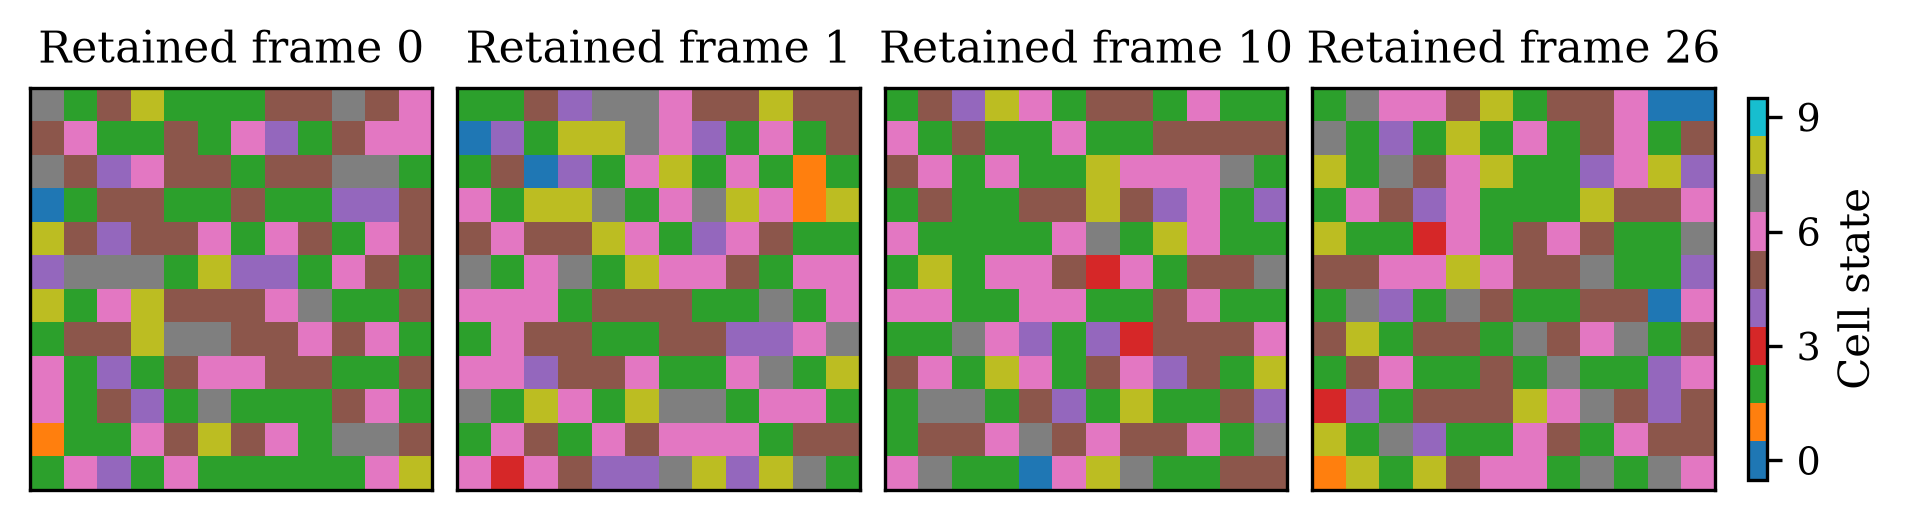
\includegraphics[width=.96\linewidth,height=3.65in,keepaspectratio]{figures/dataset.png}
\caption{Retained categorical trajectories. Actual retained validation example, row zero, frames 0, 1, 10 and 26. Colors encode categories rather than measured physical fields.}\end{figure}
\begin{figure}[htbp]\centering
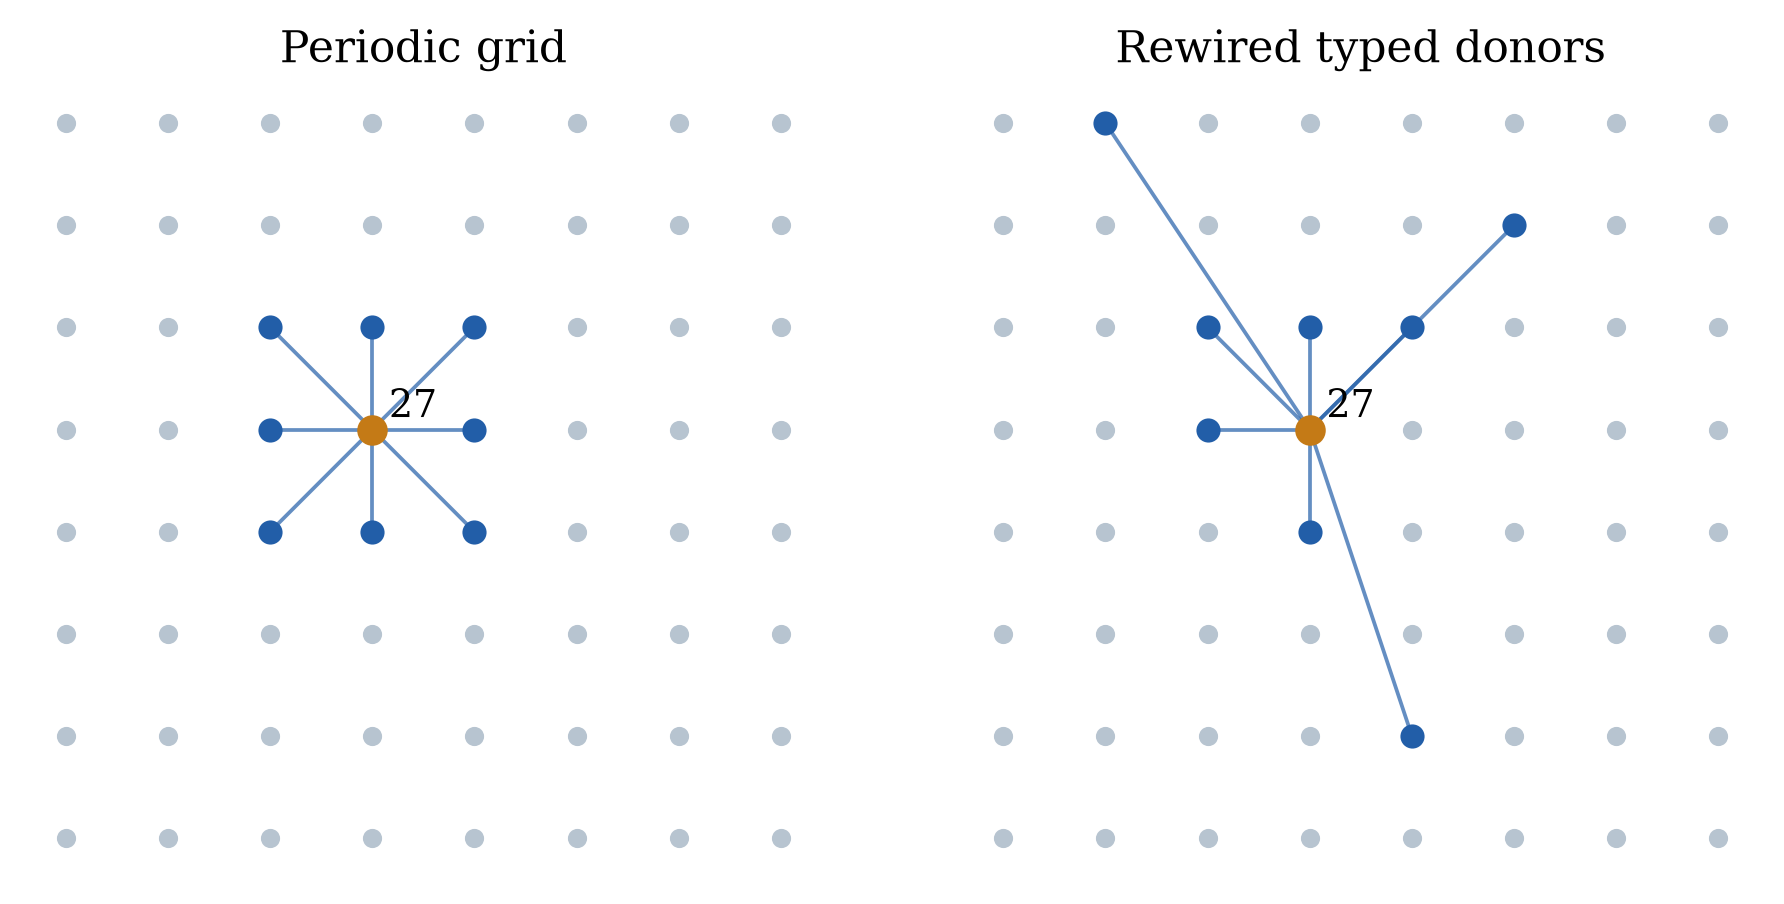
\includegraphics[width=.96\linewidth,height=3.65in,keepaspectratio]{figures/topology.png}
\caption{Actual typed grid and graph donors. The retained topology illustration compares actual donor arrays; 113 donor slots differ. This illustrative historical graph is not silently substituted for every v4 cohort.}\end{figure}
\begin{figure}[htbp]\centering
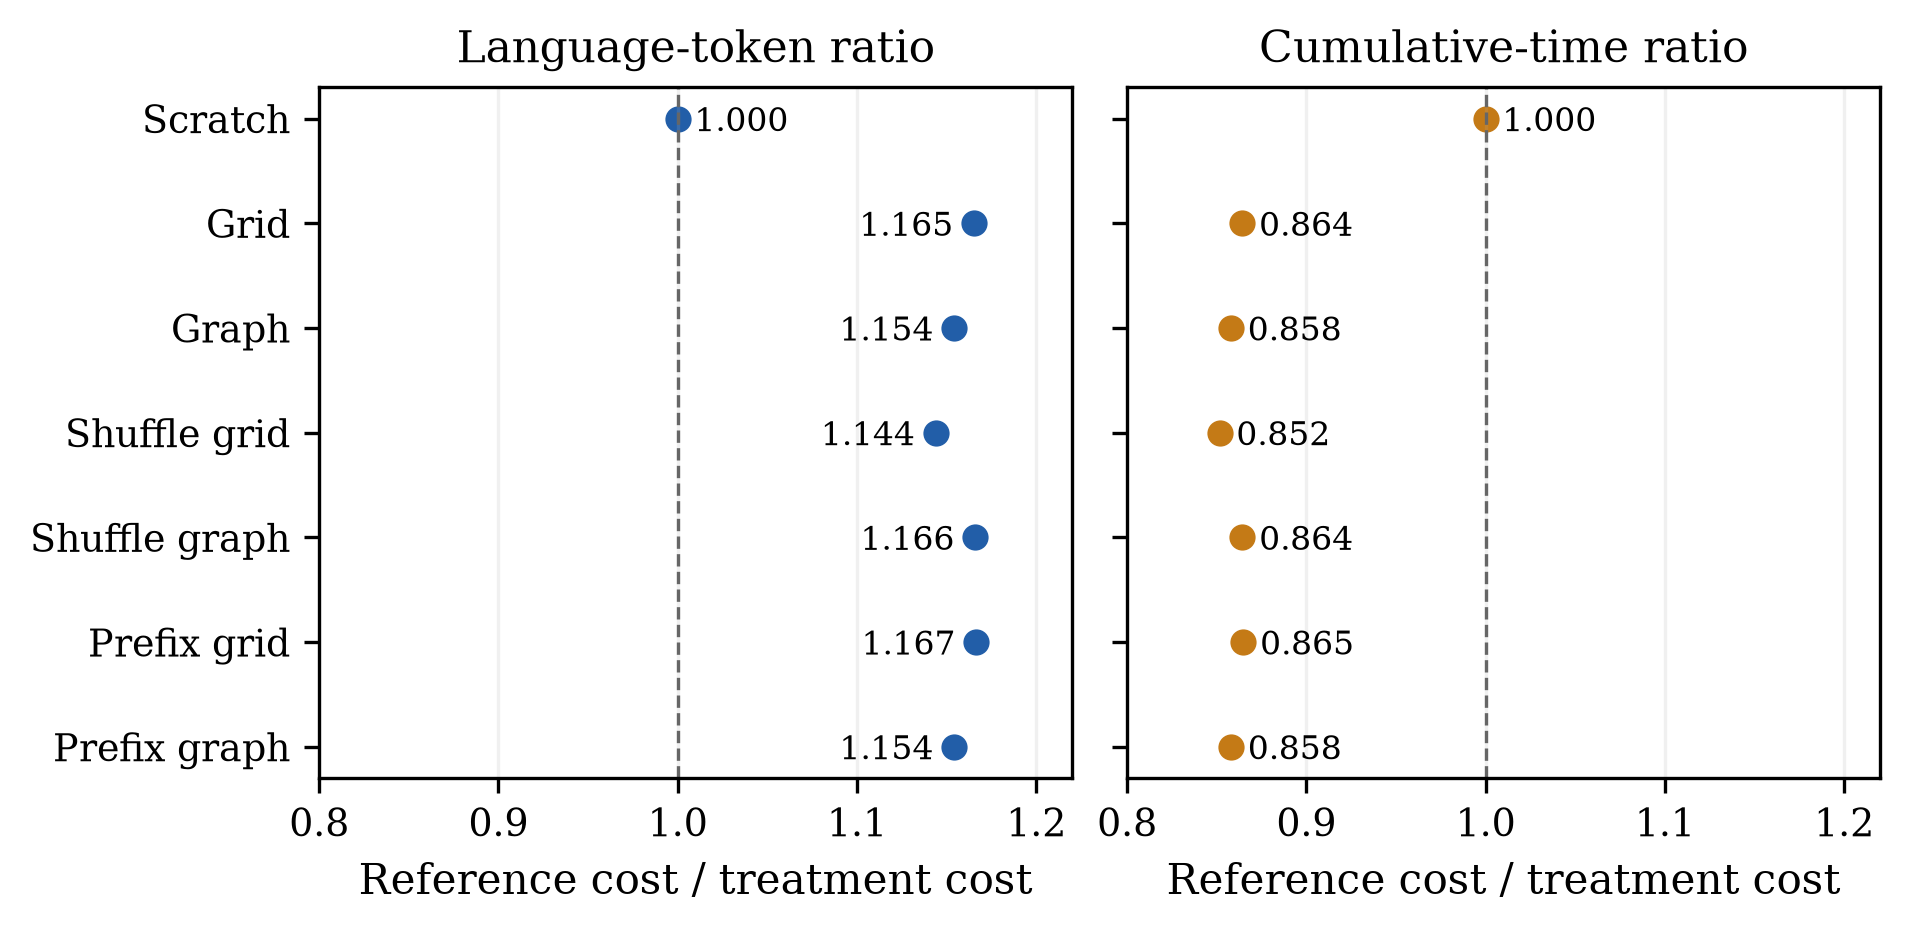
\includegraphics[width=.96\linewidth,height=3.65in,keepaspectratio]{figures/v4_cost.png}
\caption{Language transfer and cumulative cost. Recorded paired v4 ratios use different denominators for language exposure and cumulative time. A token benefit is not cumulative recovery.}\end{figure}
\begin{figure}[htbp]\centering
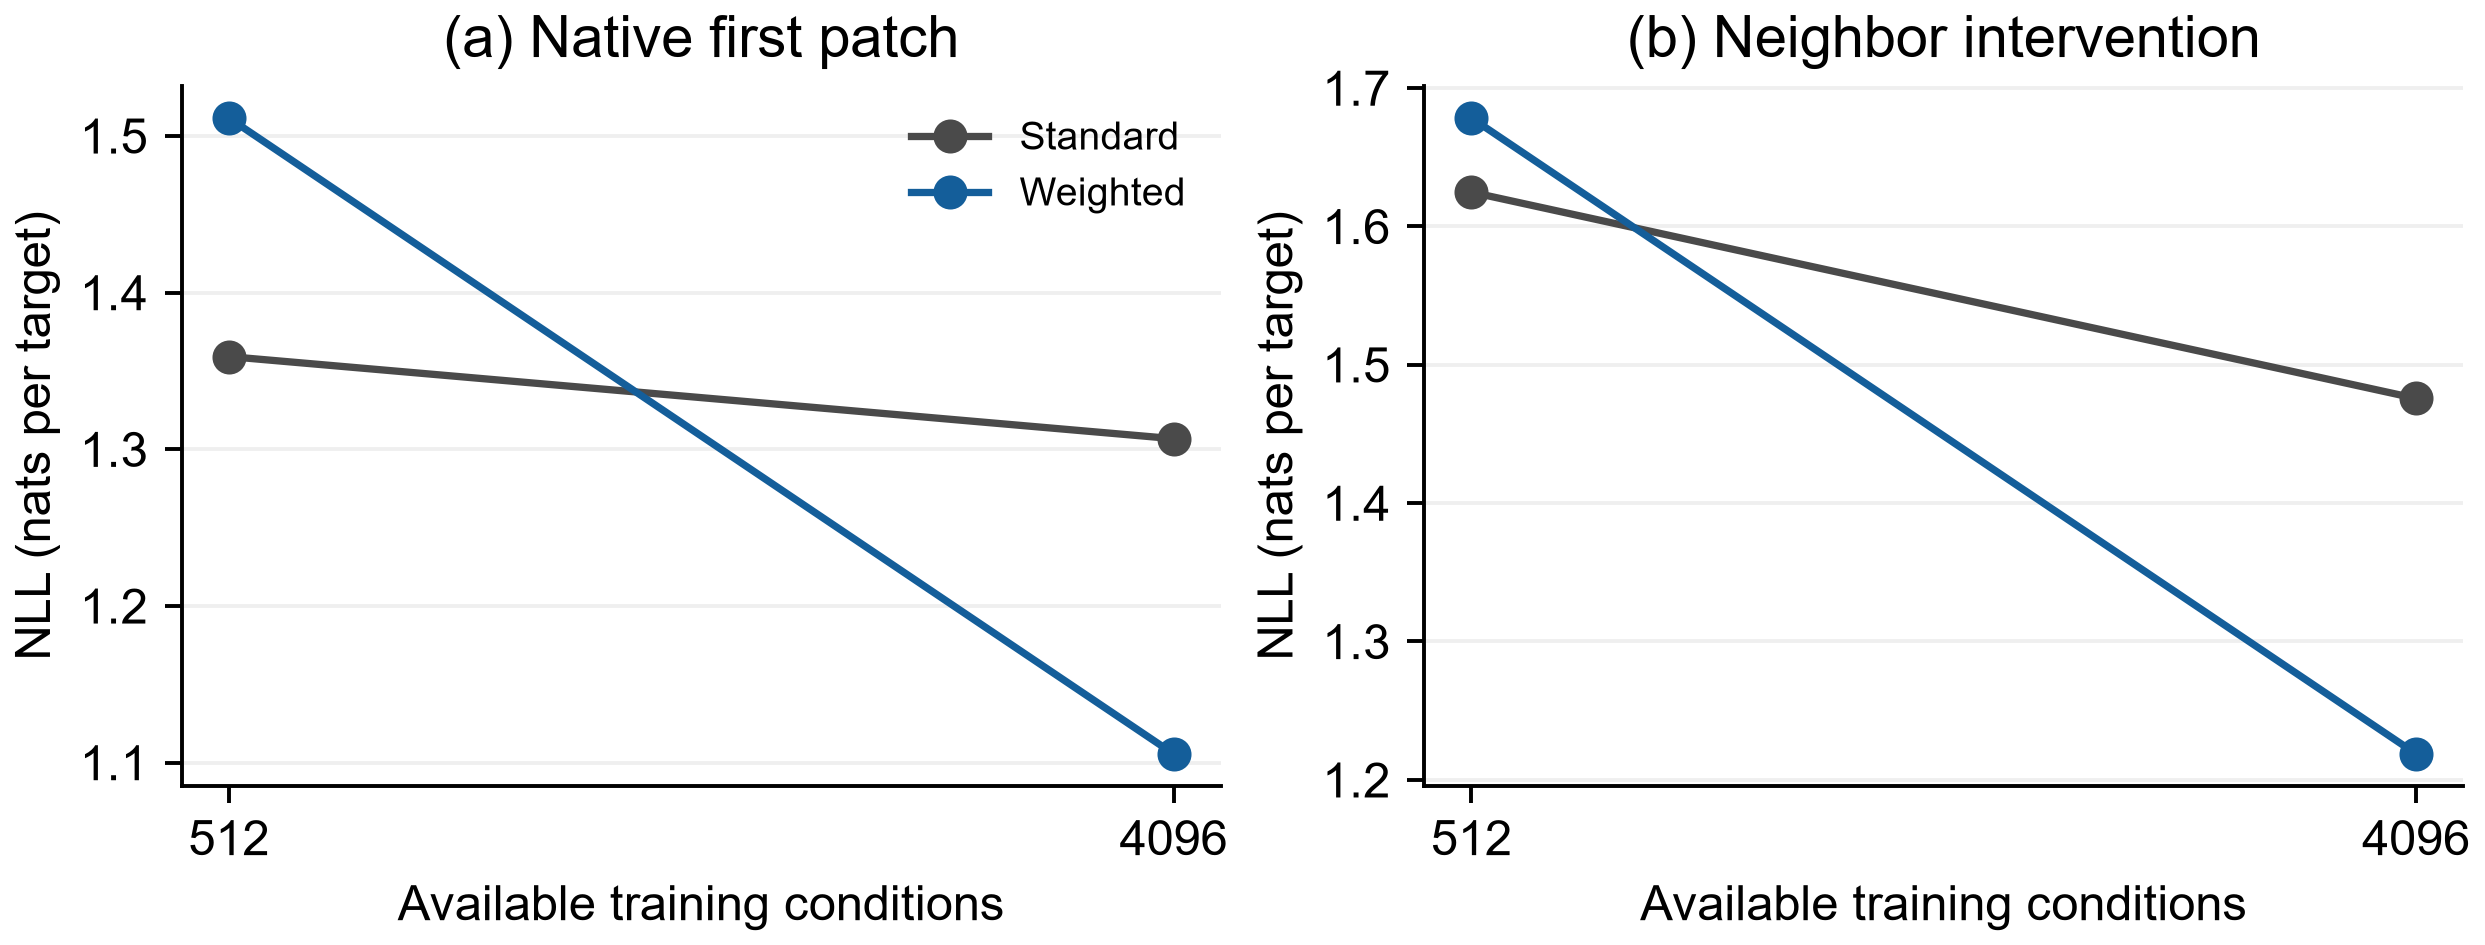
\includegraphics[width=.96\linewidth,height=3.65in,keepaspectratio]{figures/confirmation.png}
\caption{Fresh weighted and standard diversity confirmation. Three-seed endpoint NLL means. Weighted native and intervention comparisons pass all seeds; standard only one. These are fixed-budget endpoints, not speed curves.}\end{figure}
\begin{figure}[htbp]\centering
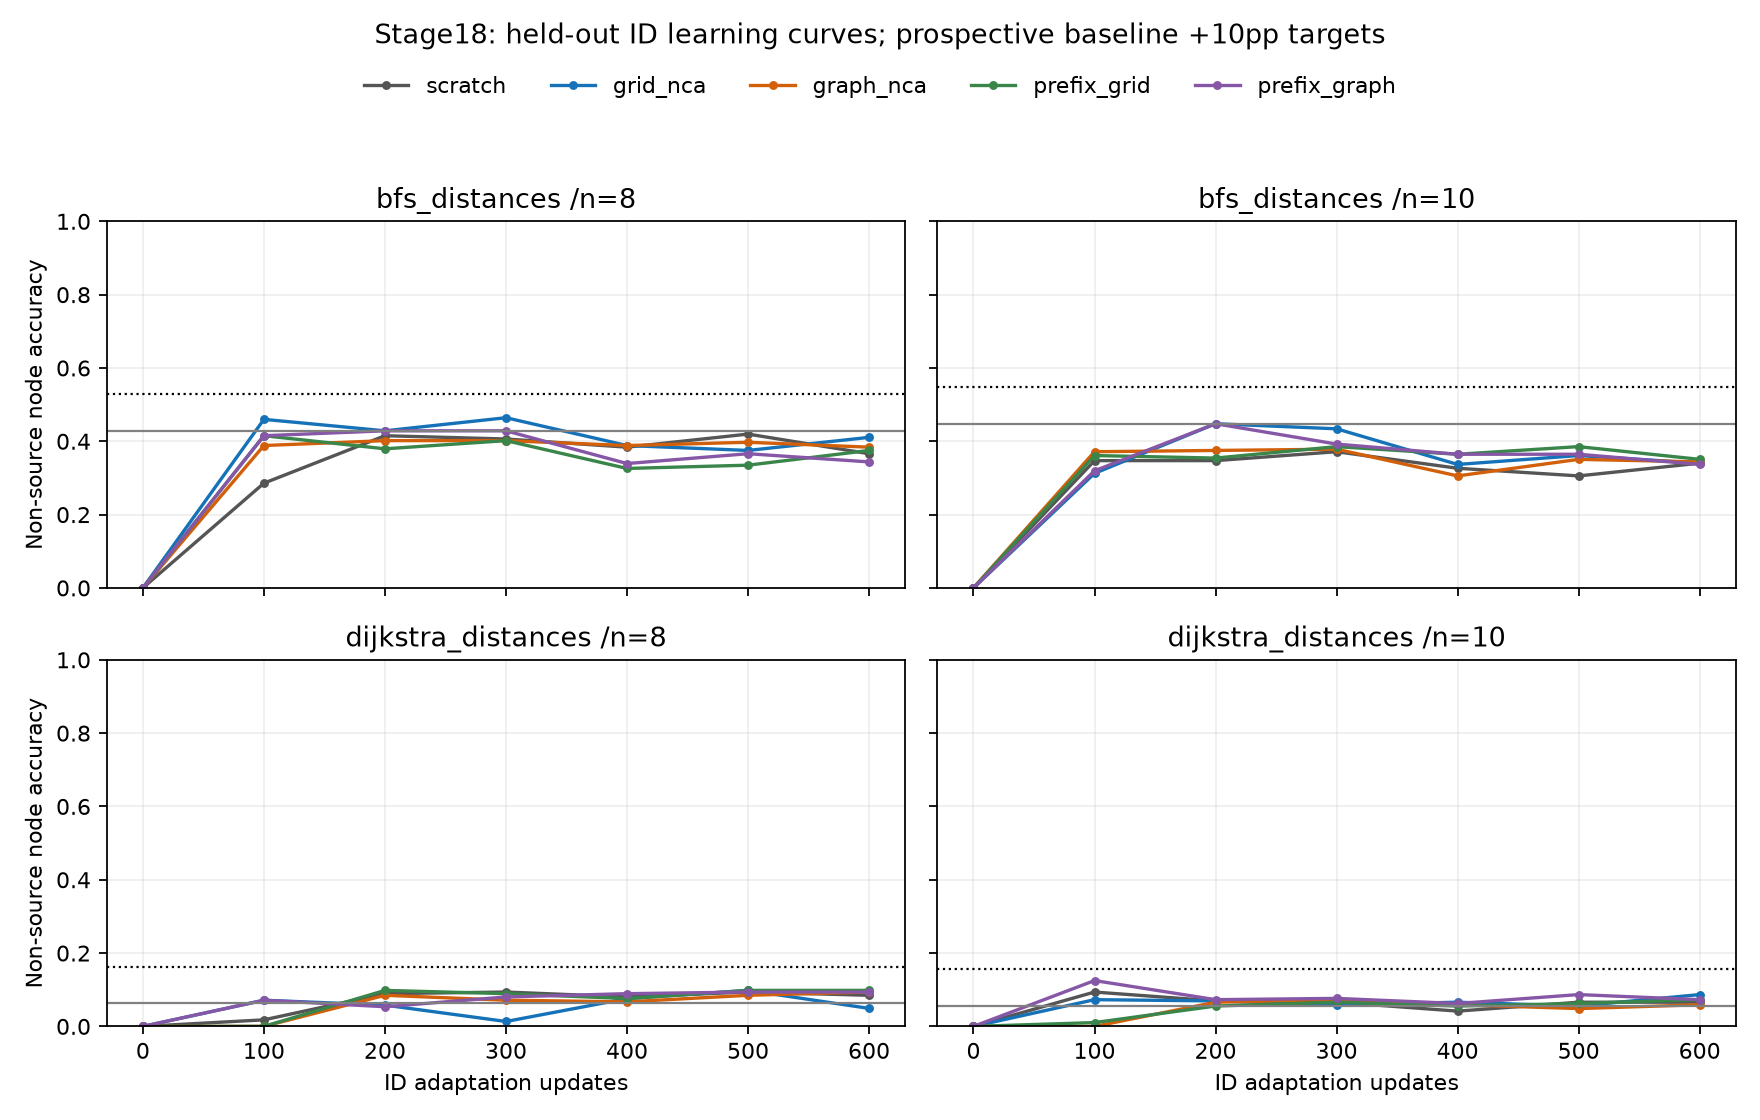
\includegraphics[width=.96\linewidth,height=3.65in,keepaspectratio]{figures/id_curves.png}
\caption{All scheduled stage 18 semantic observations. Four task/\allowbreak{}size panels preserve the source-aware marginal baseline and +10 percentage-point target. All arms remain censored at 600. Lines join observations without interpolation.}\end{figure}
\begin{figure}[htbp]\centering
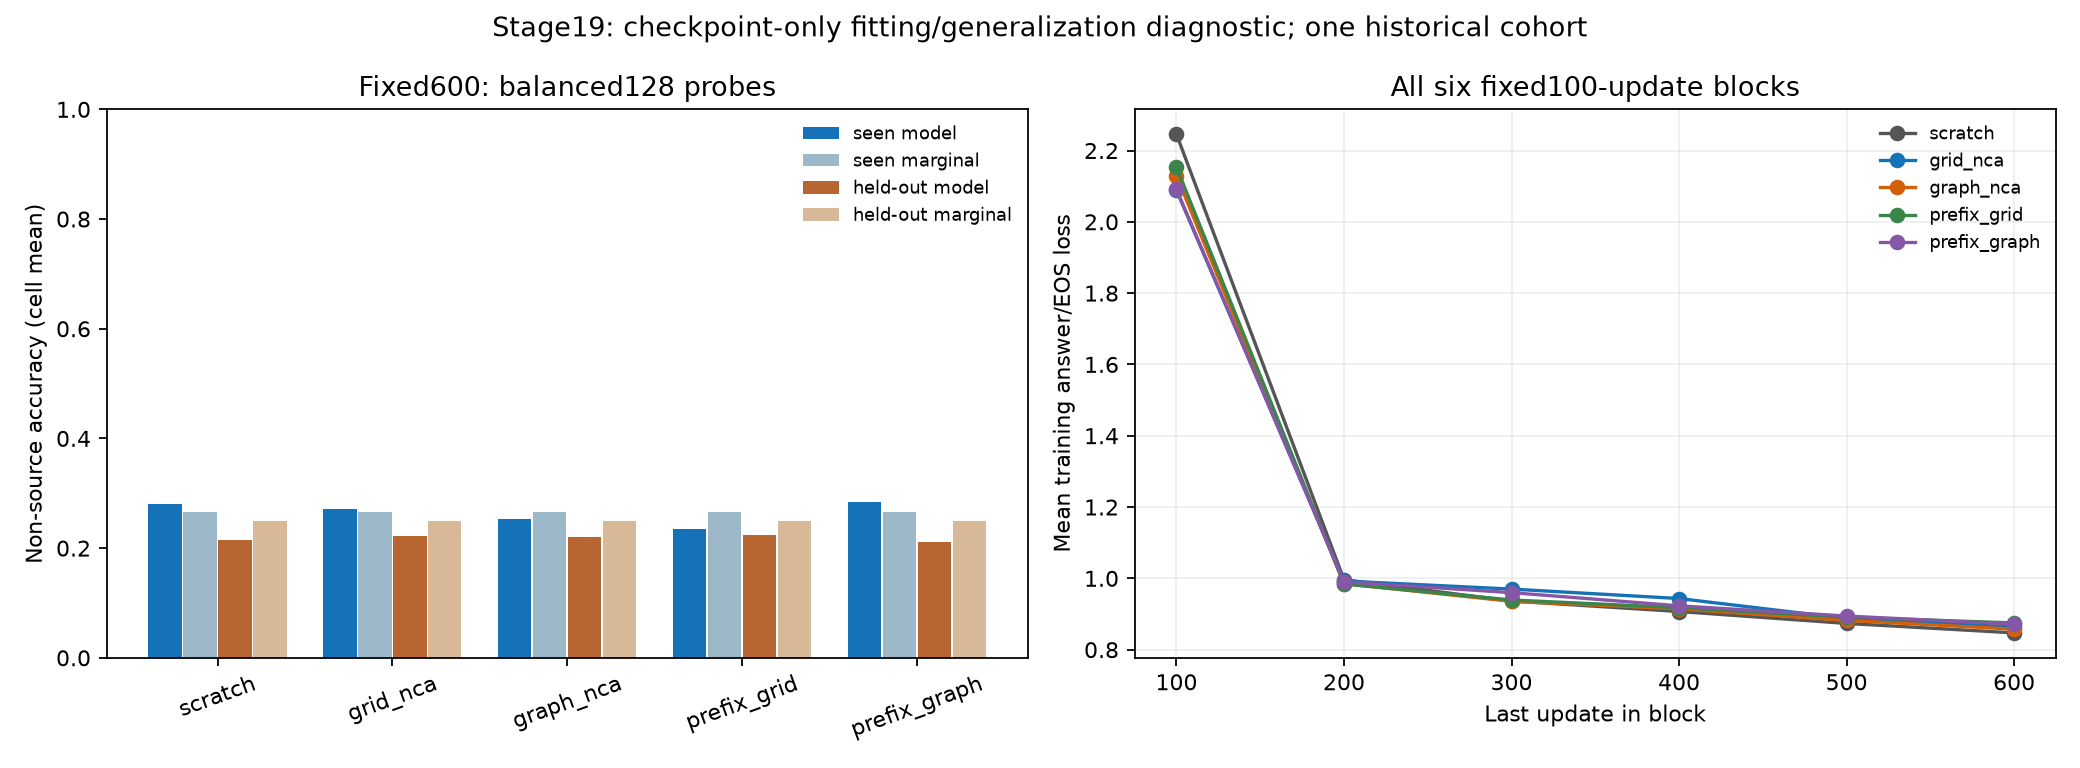
\includegraphics[width=.96\linewidth,height=3.65in,keepaspectratio]{figures/fit_and_trace.png}
\caption{Seen probe fitting and actual stage 19 trace summaries. Non-source cell means and each probe's own baseline remain separate. Six fixed block means describe optimization; they are not target crossings or a causal diagnosis.}\end{figure}
\begin{figure}[htbp]\centering
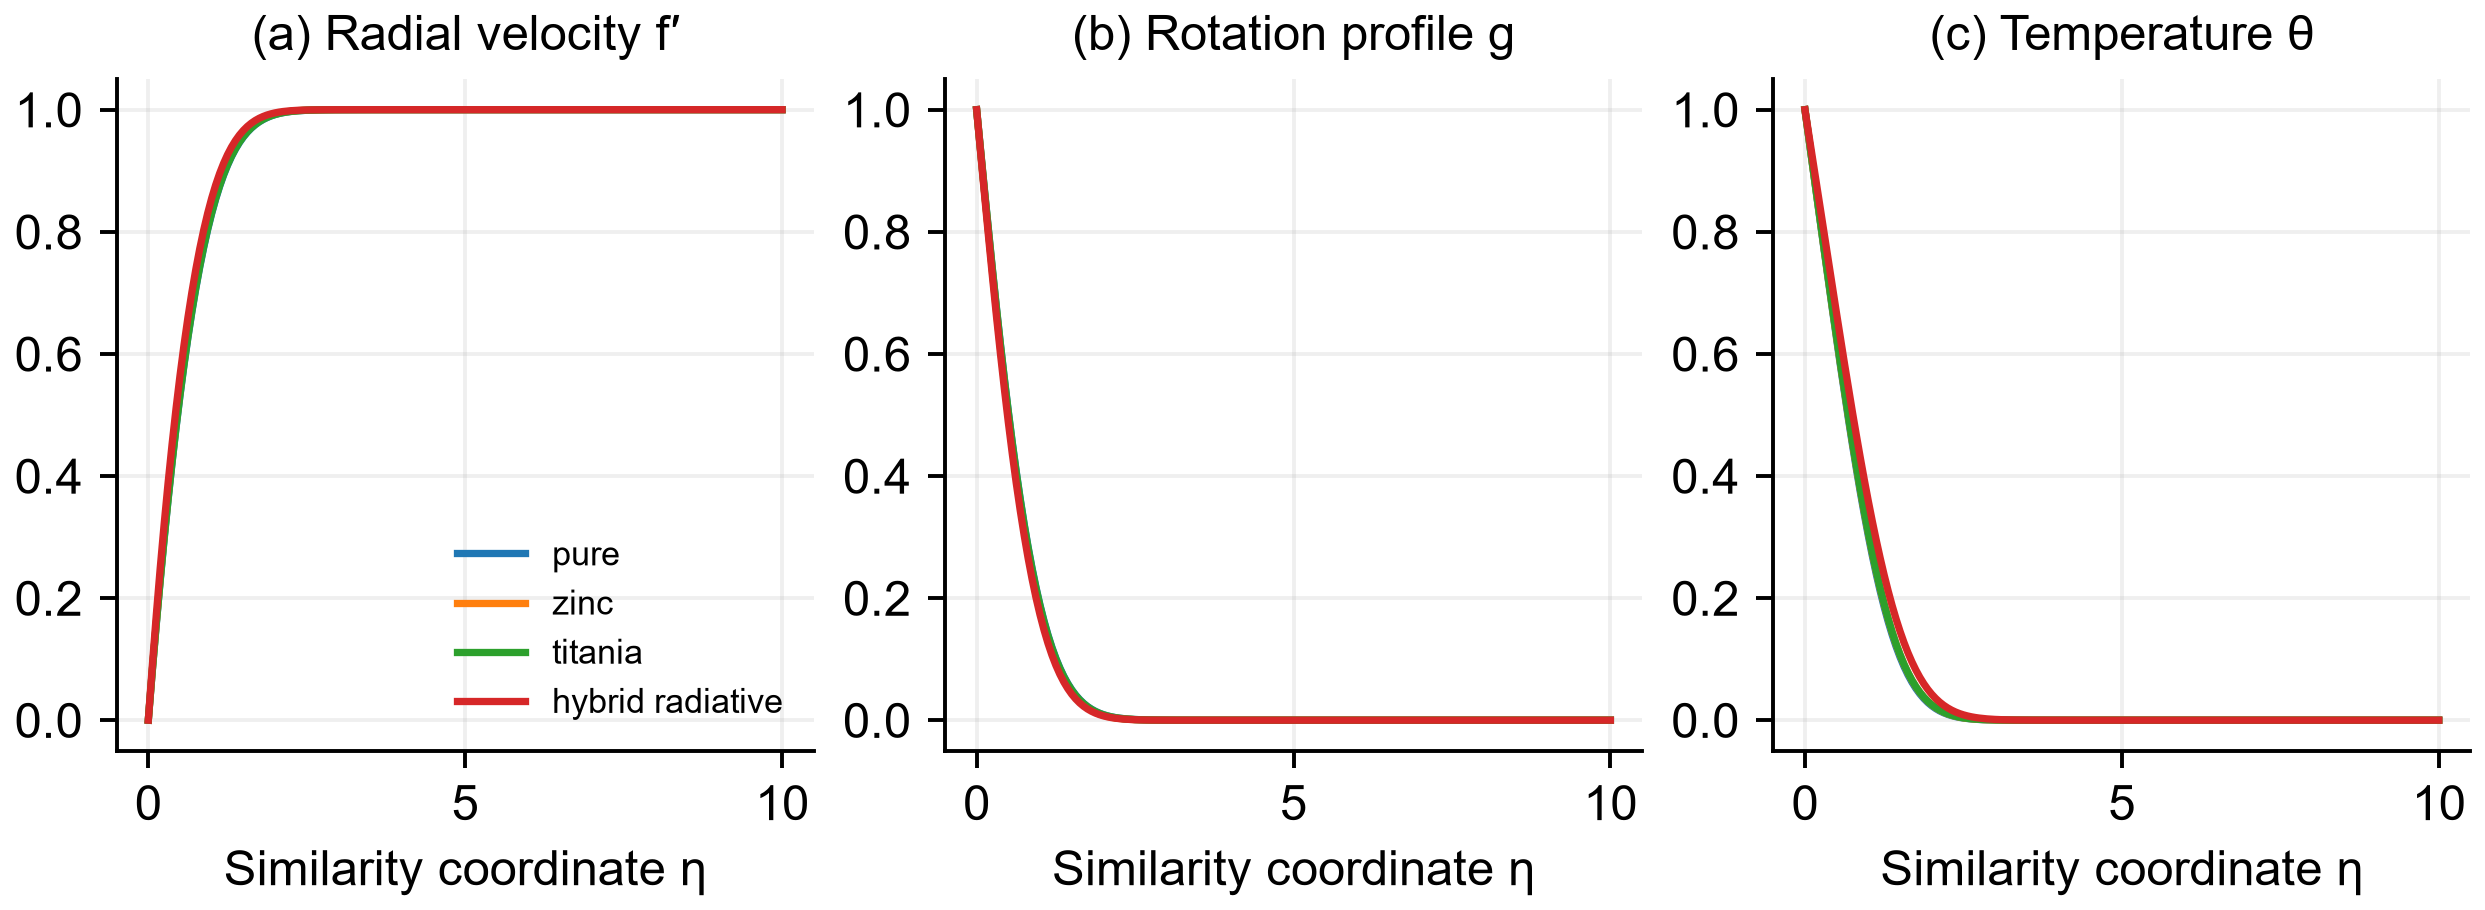
\includegraphics[width=.96\linewidth,height=3.65in,keepaspectratio]{figures/scientific_profiles.png}
\caption{Retained steady hybrid reference profiles. Profiles come directly from the four retained collocation states. They are numerical solutions of the declared steady model, not experimental data or neural predictions.}\end{figure}
\section*{References}
[1] D. Lee, S. Han, A. Kumar and P. Agrawal. Training Language Models via Neural Cellular Automata. arXiv:2603.10055v1, 2026. \url{https://arxiv.org/abs/2603.10055v1}\par
[2] A. Mordvintsev, E. Randazzo, E. Niklasson and M. Levin. Growing Neural Cellular Automata. Distill, 2020. doi:10.23915/\allowbreak{}distill.00023. \url{https://distill.pub/2020/growing-ca/}\par
[3] J. Gilmer, S. S. Schoenholz, P. F. Riley, O. Vinyals and G. E. Dahl. Neural Message Passing for Quantum Chemistry. arXiv:1704.01212, 2017. \url{https://arxiv.org/abs/1704.01212}\par
[4] A. Vaswani et al. Attention Is All You Need. arXiv:1706.03762, 2017. \url{https://arxiv.org/abs/1706.03762}\par
[5] S. Merity, C. Xiong, J. Bradbury and R. Socher. Pointer Sentinel Mixture Models. arXiv:1609.07843, 2016. \url{https://arxiv.org/abs/1609.07843}\par
[6] D. P. Kingma and J. Ba. Adam: A Method for Stochastic Optimization. arXiv:1412.6980, 2014. \url{https://arxiv.org/abs/1412.6980}\par
[7] Lean community. Theorem Proving in Lean 4. Official online documentation, accessed 20 October 2026. \url{https://lean-lang.org/theorem_proving_in_lean4/}\par
[8] S. Deb, ``Graph neural cellular automata research protocols, mathematical notes and audited evidence through stage 19,'' unpublished accompanying research bundle, Nov. 2026.\par
[9] L. Markeeva et al., ``The CLRS-Text Algorithmic Reasoning Language Benchmark,'' arXiv:2406.04229v1, 2024. \url{https://arxiv.org/abs/2406.04229v1}\par
[10] SciPy community, ``scipy.integrate.solve\_\allowbreak{}bvp,'' official documentation, accessed Nov. 2, 2026. Residual-controlled collocation method. \url{https://docs.scipy.org/doc/scipy/reference/generated/scipy.integrate.solve_bvp.html}\par
\end{document}
